\documentclass[conference]{IEEEtran}

\usepackage[T1]{fontenc}
\usepackage[utf8]{inputenc}
\usepackage{cite}
\usepackage{amsmath,amssymb,amsfonts}
\usepackage{algorithmic}
\usepackage{graphicx}
\usepackage{stfloats}
\usepackage{placeins}
\usepackage{textcomp}
\usepackage{xcolor}
\usepackage{booktabs}
\usepackage{array}
\usepackage{multirow}
\usepackage{url}
\usepackage{tikz}
\usetikzlibrary{positioning,arrows.meta,fit}
\usepackage[hidelinks]{hyperref}
\graphicspath{{figures/}}

\newcommand{\method}{U-MoE}
\newcommand{\viewset}{\mathcal{V}}
\raggedbottom
% Suggested figure slots:
% Fig. 1: Overall U-MoE architecture, drawn directly with TikZ.
% Fig. 2: Representative candlestick/image examples. Upload figures/candlestick_examples.png or replace it with your own K-line sample.
% Fig. 3: Mean expert gate weights from U-MoE, stored as figures/gate_weights_umoe.png.
% Fig. 4: Grad-CAM explanation example, stored as figures/gradcam_umoe_aapl.png.
% Fig. 5: Optional second Grad-CAM or failure case, stored as figures/gradcam_umoe_amd.png.

\begin{document}

\title{Uncertainty-aware Multi-view Expert Fusion for Interpretable Candlestick Image Trend Classification}

\author{
\IEEEauthorblockN{Author Name}
\IEEEauthorblockA{
Affiliation \\
Email: author@example.com}
}

\maketitle

\begin{abstract}
Candlestick-chart images provide a visually intuitive representation of financial time series and have been increasingly used for stock trend classification. However, high accuracy in chart-image classification is often difficult to interpret: a model may recognize the trend already visible inside the input window rather than predict subsequent price movement, and standard feature-fusion models provide limited insight into which technical views support a decision. This paper studies candlestick image trend classification from the perspective of interpretable multi-expert prediction. We propose \emph{Uncertainty-aware Multi-view Expert Fusion} (\method), which treats different technical chart renderings as view-specific image experts. Each stock window is rendered into four pure image views: raw candlestick, moving-average candlestick, RSI, and MACD. A shared ResNet18 encoder extracts view-level visual representations, each expert produces a class distribution, and an entropy-aware gating module dynamically fuses expert predictions. Experiments under strict chronological splits show a clear distinction between visible trend recognition and future direction prediction. A reproduced paper-style window-trend classifier reaches 98.37\% test accuracy, whereas strict next-day prediction remains near random. On the window-trend task, black-box concat fusion achieves the highest raw accuracy of 98.12\%, while \method{} reaches 96.74\% accuracy with explicit view-level expert weights and uncertainty estimates. On next-day prediction, \method{} does not improve accuracy, but its expert entropies approach maximum binary entropy, revealing that the model cannot identify reliable visual evidence for the future label. These results show that candlestick images are effective for recognizing visible trend structures, while \method{} provides an interpretable mechanism for diagnosing which chart views contribute to a prediction and when the prediction is uncertain.
\end{abstract}

\begin{IEEEkeywords}
Candlestick chart, financial image analysis, mixture of experts, uncertainty estimation, interpretable machine learning, multi-view learning, Grad-CAM.
\end{IEEEkeywords}

\section{Introduction}

Financial time-series prediction is challenging because asset prices are noisy, non-stationary, and affected by latent market mechanisms that are only partially observable \cite{rouf2021stocksurvey,meng2021urts}. In recent years, an alternative to numerical feature engineering has gained attention: converting historical price windows into candlestick-chart images and applying computer vision models to classify market trends \cite{kusuma2019deepcandle,pizon2025image}. Candlestick charts are appealing because they encode open, high, low, and close prices in a compact visual format familiar to market participants \cite{mersal2023systematic}.

Despite promising reported results in chart-image and object-recognition-based trading systems \cite{nguyen2023object,temur2024comparison}, image-based stock prediction raises two important questions. First, what exactly is being predicted? In many chart-image settings, the label describes whether the displayed window itself moves upward or downward. A model can then obtain high accuracy by recognizing a trend already visible inside the input image. This is a legitimate visual trend recognition task, but it differs from predicting the next trading day's price direction. Second, when a model uses multiple technical chart views, such as candlesticks, moving averages, RSI, and MACD, how can we know which view contributes to the final decision? Standard feature concatenation can be accurate, but it provides little view-level interpretability.

This paper focuses on interpretable pure-image trend classification while explicitly controlling for the distinction between visible trend recognition and future prediction. Our central hypothesis is that different technical image views behave like distinct experts: candlesticks capture price body and wick patterns, moving averages capture trend direction, RSI captures momentum saturation, and MACD captures oscillator changes. A mixture-of-experts architecture is therefore a natural fit for multi-view financial chart images \cite{jacobs1991adaptive,shazeer2017outrageous,xin2024i2moe}, provided that the model can also quantify expert uncertainty.

We propose \method{}, a multi-view image model in which each chart view has an expert classifier and a gate dynamically aggregates expert predictions. Fig.~\ref{fig:method-overview} summarizes the proposed framework. Unlike ordinary MoE models that rely only on learned gate scores, \method{} discounts experts with high predictive entropy. This design produces not only a final class probability, but also interpretable quantities: expert probabilities, expert entropies, and gate weights. These quantities allow us to ask whether the model relies more on candlestick, moving-average, RSI, or MACD views, and whether the decision is supported by confident or uncertain experts.

The main contributions are:
\begin{itemize}
    \item We formulate a pure-image multi-view candlestick trend classification setting in which candle, moving-average, RSI, and MACD charts are treated as view-specific experts.
    \item We propose \method{}, an uncertainty-aware mixture-of-experts fusion method that combines expert predictions using entropy-regularized view weights.
    \item We show that \method{} provides explicit view-level interpretability through expert weights and predictive entropies, while retaining strong trend-recognition performance.
    \item We empirically distinguish visible window-trend recognition from strict next-day prediction and show that \method{} can diagnose prediction failure through high expert uncertainty.
\end{itemize}

\section{Related Work}

\subsection{Candlestick Image Classification}
Candlestick charts summarize price action through visual primitives such as candle bodies, shadows, gaps, and trend slopes \cite{mersal2023systematic}. Recent studies transform financial time-series windows into chart images and apply convolutional neural networks, object recognition methods, or image classification architectures to identify trend or pattern classes \cite{kusuma2019deepcandle,pizon2025image,nguyen2023object,temur2024comparison}. These methods demonstrate that visual encodings can be useful for learning chart structures. However, reported high accuracies often depend strongly on label definition, window construction, and split protocol. If the target label is derived from the same window displayed in the input image, the task is trend recognition rather than future prediction.

\subsection{Multi-view Financial Representations}
Financial market states can be represented from multiple perspectives: raw price charts, moving-average overlays, momentum oscillators, volatility indicators, and volume patterns. Multi-view and multimodal time-series learning provide principled ways to combine complementary observations \cite{jiang2025multimodal,wang2026multiview}. Related financial work has also explored latent-space retrieval and multi-resolution market information \cite{bamford2023retrieval,farimani2025contrastive}. In this paper, we restrict all information to rendered images, avoiding numerical tabular features or text modalities. This allows us to study whether a pure image model can learn and explain trend-related visual structures from multiple technical chart views.

\subsection{Mixture of Experts and Uncertainty}
Mixture-of-experts models decompose prediction into multiple specialized experts and a gating network that assigns input-dependent expert weights \cite{jacobs1991adaptive,shazeer2017outrageous}. Recent interpretable multimodal MoE work further shows that expert weighting can expose sample-level and dataset-level interaction patterns \cite{xin2024i2moe}. In financial chart analysis, different technical indicators may be informative under different market conditions. Uncertainty estimation is also important because a model's lack of confidence can be as informative as its predicted class \cite{guo2017calibration}. We use predictive entropy to discount uncertain experts and to diagnose whether individual chart views provide reliable evidence.



\section{Problem Definition}

\subsection{Data Setting}
We use daily OHLC data from ten U.S. stocks: AAPL, TSLA, MSFT, AMZN, NVDA, META, GOOG, JPM, AMD, and BAC. The historical period spans from 20 February 2020 to 18 December 2023. Each sample is constructed from a 30-trading-day window. The dataset contains 5,283 samples split chronologically into 3,667 training samples, 818 validation samples, and 798 test samples. The chronological split avoids placing highly overlapping windows from nearby dates into both training and test sets.

\subsection{Label Definitions}
We consider two labels. The \emph{window-trend} label is
\begin{equation}
y_i^{\mathrm{win}} = \mathbb{1}(C_t > C_{t-29}),
\end{equation}
where $C_t$ is the closing price at the end of the input window and $C_{t-29}$ is the closing price at the start of the same 30-day window. This label measures whether the input chart itself displays an upward or downward trend.

The \emph{next-day} label is
\begin{equation}
y_i^{\mathrm{next}} = \mathbb{1}(C_{t+1} > C_t).
\end{equation}
This label is outside the input window and corresponds to strict next-trading-day direction prediction. Window-trend classification evaluates visual trend recognition, whereas next-day classification evaluates whether the image contains predictive information for the immediate future.

\subsection{Multi-view Image Inputs}
For each window, we render four RGB image views:
\begin{itemize}
    \item $x^{\mathrm{candle}}$: raw candlestick chart.
    \item $x^{\mathrm{MA}}$: candlestick chart with moving-average overlays.
    \item $x^{\mathrm{RSI}}$: relative strength index chart.
    \item $x^{\mathrm{MACD}}$: MACD histogram and signal-line chart.
\end{itemize}
No numerical OHLC values, volume features, text, news, or tabular technical indicators are provided to the model. All technical information is visible only through images. Fig.~\ref{fig:candlestick-examples} shows real multi-view samples from the AutoDL dataset.
\begin{figure*}[!t]
\centering

\includegraphics[width=0.92\textwidth]{candlestick_multiview_samples.png}
\caption{Real multi-view candlestick image samples from the AutoDL dataset. Each row corresponds to one 30-trading-day stock window, and columns show the candlestick, MA, RSI, and MACD views used by the four experts.}
\label{fig:candlestick-examples}
\end{figure*}

\section{Method}
\begin{figure*}[!t]
\centering
\resizebox{0.98\textwidth}{!}{%
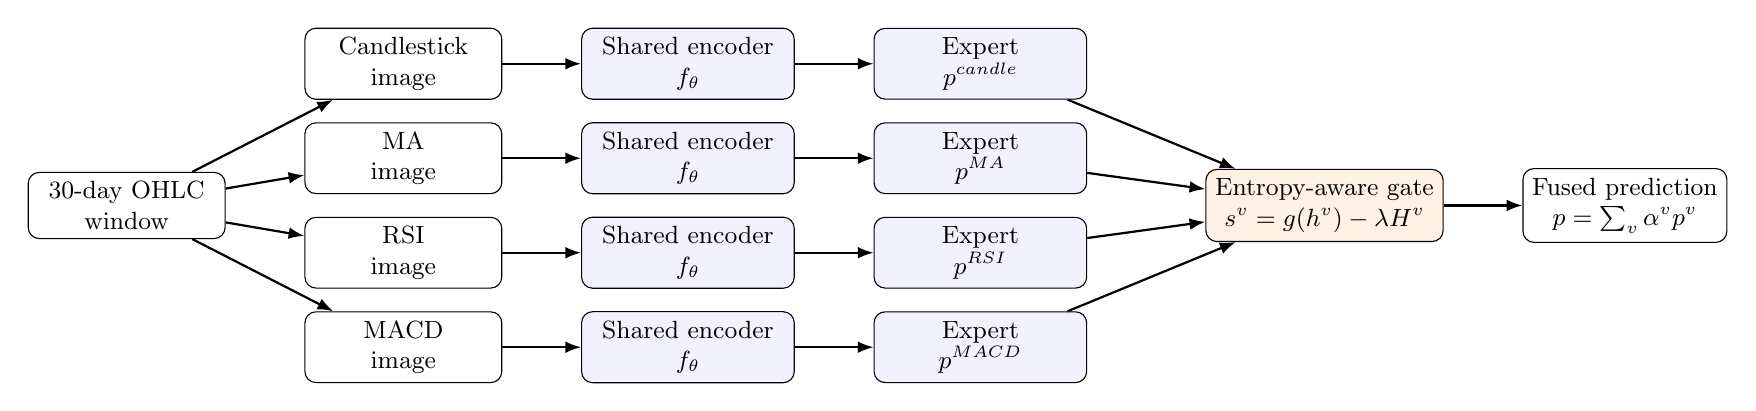
\begin{tikzpicture}[
    font=\small,
    node distance=7mm and 10mm,
    box/.style={draw, rounded corners, align=center, minimum width=25mm, minimum height=8mm},
    expert/.style={draw, rounded corners, align=center, minimum width=27mm, minimum height=8mm, fill=blue!5},
    gate/.style={draw, rounded corners, align=center, minimum width=30mm, minimum height=8mm, fill=orange!10},
    arrow/.style={-{Latex[length=2mm]}, thick}
]
\node[box] (input) {30-day OHLC\\window};
\node[box, right=of input, yshift=18mm] (candle) {Candlestick\\image};
\node[box, right=of input, yshift=6mm] (ma) {MA\\image};
\node[box, right=of input, yshift=-6mm] (rsi) {RSI\\image};
\node[box, right=of input, yshift=-18mm] (macd) {MACD\\image};

\node[expert, right=of candle] (ec) {Shared encoder\\$f_\theta$};
\node[expert, right=of ma] (em) {Shared encoder\\$f_\theta$};
\node[expert, right=of rsi] (er) {Shared encoder\\$f_\theta$};
\node[expert, right=of macd] (ed) {Shared encoder\\$f_\theta$};

\node[expert, right=of ec] (pc) {Expert\\$p^{candle}$};
\node[expert, right=of em] (pm) {Expert\\$p^{MA}$};
\node[expert, right=of er] (pr) {Expert\\$p^{RSI}$};
\node[expert, right=of ed] (pd) {Expert\\$p^{MACD}$};

\node[gate, right=15mm of pm, yshift=-6mm] (gate) {Entropy-aware gate\\$s^v=g(h^v)-\lambda H^v$};
\node[box, right=of gate] (out) {Fused prediction\\$p=\sum_v \alpha^v p^v$};

\draw[arrow] (input) -- (candle); \draw[arrow] (input) -- (ma); \draw[arrow] (input) -- (rsi); \draw[arrow] (input) -- (macd);
\draw[arrow] (candle) -- (ec); \draw[arrow] (ma) -- (em); \draw[arrow] (rsi) -- (er); \draw[arrow] (macd) -- (ed);
\draw[arrow] (ec) -- (pc); \draw[arrow] (em) -- (pm); \draw[arrow] (er) -- (pr); \draw[arrow] (ed) -- (pd);
\draw[arrow] (pc) -- (gate); \draw[arrow] (pm) -- (gate); \draw[arrow] (pr) -- (gate); \draw[arrow] (pd) -- (gate);
\draw[arrow] (gate) -- (out);
\end{tikzpicture}%
}
\caption{Overview of the proposed uncertainty-aware multi-view expert fusion framework. Each technical chart view is encoded by a shared visual encoder, classified by a view-specific expert, and combined through an entropy-aware gate. The final prediction is decomposable into expert beliefs, expert uncertainties, and gate weights.}
\label{fig:method-overview}
\end{figure*}

\subsection{Shared Visual Encoder}
Let $\viewset=\{1,\ldots,M\}$ denote the set of views, with $M=4$. For sample $i$, view $v$ is an image $x_i^v$. A shared ResNet18 encoder $f_\theta$ maps each view to a feature vector:
\begin{equation}
h_i^v = f_\theta(x_i^v) \in \mathbb{R}^{d}.
\end{equation}
The encoder is initialized from ImageNet weights and can optionally be initialized from a multi-view consistency pretraining checkpoint. The same encoder is shared across views to encourage a common visual representation space.

\subsection{View-specific Experts}
Each view has an expert classifier $E_v$. The expert produces logits and probabilities:
\begin{equation}
z_i^v = W_v h_i^v + b_v,
\end{equation}
\begin{equation}
p_i^v = \mathrm{softmax}(z_i^v).
\end{equation}
The expert prediction $p_i^v$ can be interpreted as the class belief of a specific technical chart view.

\subsection{Expert Uncertainty}
For each expert, we compute predictive entropy:
\begin{equation}
H_i^v = -\sum_{c=1}^{K} p_i^v(c)\log p_i^v(c),
\end{equation}
where $K=2$ for binary trend classification. Entropy is high when an expert assigns similar probabilities to upward and downward classes. In binary classification, the maximum entropy is $\log 2 \approx 0.693$.

\subsection{Uncertainty-aware Gating}
The gate produces an input-dependent score for each expert. In the local-gate variant, the score is computed from each view feature:
\begin{equation}
a_i^v = g_\psi(h_i^v).
\end{equation}
In the uncertainty-aware version, the score is penalized by expert entropy:
\begin{equation}
s_i^v = a_i^v - \lambda H_i^v,
\end{equation}
where $\lambda$ controls the strength of uncertainty discounting. Gate weights are obtained by a softmax over views:
\begin{equation}
\alpha_i^v = \frac{\exp(s_i^v)}{\sum_{u=1}^{M}\exp(s_i^u)}.
\end{equation}
The final \method{} prediction is a weighted average of expert probabilities:
\begin{equation}
p_i^{\mathrm{MoE}} = \sum_{v=1}^{M}\alpha_i^v p_i^v.
\end{equation}
This formulation makes the prediction decomposable. The final probability is determined by expert beliefs $p_i^v$, expert uncertainty $H_i^v$, and gate weights $\alpha_i^v$.

\subsection{Residual Concat Branch}
We also evaluate a residual version that combines \method{} with a standard concat-fusion classifier:
\begin{equation}
h_i^{\mathrm{cat}} = [h_i^1;h_i^2;\ldots;h_i^M],
\end{equation}
\begin{equation}
p_i^{\mathrm{cat}} = \mathrm{softmax}(q_\omega(h_i^{\mathrm{cat}})).
\end{equation}
The residual prediction is
\begin{equation}
p_i = (1-\rho)p_i^{\mathrm{MoE}} + \rho p_i^{\mathrm{cat}}.
\end{equation}
This variant tests whether a black-box concat branch can improve performance while preserving expert weights for interpretation.

\subsection{Training Objective}
The main classification loss is the negative log-likelihood of the fused prediction:
\begin{equation}
\mathcal{L}_{\mathrm{cls}} = -\log p_i(y_i).
\end{equation}
We also include an auxiliary expert loss:
\begin{equation}
\mathcal{L}_{\mathrm{aux}} = \frac{1}{M}\sum_{v=1}^{M}\mathrm{CE}(z_i^v,y_i),
\end{equation}
which encourages each expert to remain individually predictive. A consistency term aligns expert distributions with the fused prediction:
\begin{equation}
\mathcal{L}_{\mathrm{cons}} = \frac{1}{M}\sum_{v=1}^{M}\mathrm{KL}(p_i \parallel p_i^v).
\end{equation}
The total loss is
\begin{equation}
\mathcal{L} =
\mathcal{L}_{\mathrm{cls}}
+ \beta\mathcal{L}_{\mathrm{aux}}
+ \eta\mathcal{L}_{\mathrm{cons}}
+ \gamma\mathcal{L}_{\mathrm{div}},
\end{equation}
where $\mathcal{L}_{\mathrm{div}}$ is an optional feature-diversity regularizer.

\section{Experimental Setup}

\subsection{Baselines}
We compare \method{} with the following baselines:
\begin{itemize}
    \item \textbf{Lightweight CNN}: a reproduction baseline for single candlestick-image classification.
    \item \textbf{Mean fusion}: average of four view embeddings followed by a classifier.
    \item \textbf{Concat fusion}: concatenation of four view embeddings followed by an MLP classifier.
    \item \textbf{Regularized concat}: concat fusion with stronger dropout, data augmentation, label smoothing, and weight decay.
    \item \textbf{Frozen encoder probe}: encoder frozen, classifier trained on downstream labels.
    \item \textbf{Shuffled-label sanity check}: training labels randomly permuted while validation and test labels remain true.
\end{itemize}
Concat fusion is the strongest accuracy baseline but is not our proposed contribution. It is included to test whether interpretability comes at a performance cost.

\subsection{Metrics}
We report accuracy, weighted F1, confusion matrices, and class-level reports. For representation quality, we report retrieval Hit@1 using cosine similarity between learned features, following the intuition that useful representations should organize visually similar financial windows in latent space \cite{bamford2023retrieval}. For interpretability, we analyze expert gate weights, expert entropies, and Grad-CAM heatmaps \cite{selvaraju2017gradcam}.

\section{Results}

\subsection{Window-trend Recognition vs. Next-day Prediction}
Table~\ref{tab:label-def} shows the effect of label definition. The same image-based setting yields very different results depending on the target. The high window-trend score indicates that the model can recognize the trend already displayed in the image. The next-day score is near random, suggesting that static chart images alone do not provide reliable immediate future-direction signals in this setting.

\begin{figure}[!t]
\centering

\includegraphics[width=\linewidth]{task_accuracy_comparison.png}
\caption{Accuracy comparison across visible window-trend recognition and strict next-day prediction. High scores occur when the target is visually encoded in the input window, while next-day prediction remains close to random.}
\label{fig:task-accuracy}
\end{figure}

\begin{table}[t]
\centering
\caption{Reproduction under different target definitions.}
\label{tab:label-def}
\begin{tabular}{llcc}
\toprule
Task & Model & Acc. & F1 \\
\midrule
Window-trend & CNN & 0.9837 & $\approx$0.9837 \\
Next-day & CNN & 0.4962 & $\approx$0.4757 \\
\bottomrule
\end{tabular}
\end{table}

\subsection{Multi-view Fusion Baselines}
Table~\ref{tab:fusion} compares multi-view fusion strategies on the window-trend task. Concat fusion achieves the best raw accuracy, confirming that view-specific information is complementary. However, concat fusion does not explicitly reveal which view contributes to a decision. \method{} addresses this interpretability gap.

\begin{table}[t]
\centering
\caption{Multi-view window-trend classification.}
\label{tab:fusion}
\begin{tabular}{lccc}
\toprule
Model & Acc. & F1 & Hit@1 \\
\midrule
Mean fusion & 0.9561 & 0.9562 & 0.9574 \\
Concat fusion & 0.9812 & 0.9813 & 0.9674 \\
Regularized concat & 0.9712 & 0.9712 & 0.9599 \\
Frozen probe & 0.9398 & 0.9400 & 0.9273 \\
\bottomrule
\end{tabular}
\end{table}

\subsection{\method{} on Window-trend Classification}
Table~\ref{tab:umoe-window} presents \method{} results on the window-trend task. The local uncertainty-aware model achieves 96.74\% accuracy with balanced expert weights. Although it does not exceed concat fusion in accuracy, it provides a direct decomposition of model behavior. The model assigns substantial weight to candlestick, MA, and RSI views, while MACD receives lower average weight.

\begin{table*}[t]
\centering
\caption{\method{} window-trend results.}
\label{tab:umoe-window}
\begin{tabular}{lcccl}
\toprule
Model & Acc. & F1 & Hit@1 & Mean gate weights \\
\midrule
Vanilla local MoE & 0.9674 & 0.9675 & 0.9712 & candle .302, MA .294, RSI .248, MACD .156 \\
Uncertainty local MoE & 0.9674 & 0.9675 & 0.9712 & candle .291, MA .289, RSI .261, MACD .159 \\
Global U-MoE regularized & 0.9574 & 0.9573 & 0.9674 & candle .167, MA .386, RSI .035, MACD .412 \\
Residual MLP U-MoE & 0.9649 & 0.9648 & 0.9662 & candle .002, MA .635, RSI .352, MACD .011 \\
\bottomrule
\end{tabular}
\end{table*}

\subsection{\method{} on Next-day Prediction}
Table~\ref{tab:next-day} evaluates whether \method{} improves strict next-day prediction. \method{} does not improve next-day prediction. This negative result is important: a more expressive interpretable fusion model does not overcome the lack of stable predictive signal in the image-only input.

\begin{table}[t]
\centering
\caption{Next-day prediction results.}
\label{tab:next-day}
\begin{tabular}{lccc}
\toprule
Model & Acc. & F1 & Hit@1 \\
\midrule
CNN & 0.4962 & 0.4757 & -- \\
MV pretrain + classifier & 0.4850 & 0.4300 & 0.4975 \\
U-MoE local uncertainty & 0.4724 & 0.4732 & 0.4987 \\
Residual MLP U-MoE & 0.4712 & 0.4305 & 0.4987 \\
\bottomrule
\end{tabular}
\end{table}

The uncertainty estimates further support this interpretation. For local \method{}, mean expert entropies are 0.6789 for candlestick, 0.6797 for MA, 0.6734 for RSI, and 0.6825 for MACD. Since the maximum binary entropy is approximately 0.693, all experts are highly uncertain. Thus, \method{} explains the failure mode: the model is not merely choosing the wrong view; all views provide weak and uncertain evidence for next-day direction.

\begin{table}[!t]
\centering
\caption{Mean expert entropy on strict next-day prediction. Values close to $\log 2 \approx 0.693$ indicate near-maximum uncertainty.}
\label{tab:nextday-entropy}
\begin{tabular}{lc}
\toprule
Expert view & Mean entropy \\
\midrule
Candlestick & 0.6789 \\
MA & 0.6797 \\
RSI & 0.6734 \\
MACD & 0.6825 \\
\bottomrule
\end{tabular}
\end{table}

\subsection{Shuffled-label Sanity Check}
The shuffled-label diagnostic in Table~\ref{tab:shuffle} substantially reduces classification performance from 98.12\% to 69.92\%. The remaining above-chance accuracy is mainly caused by class imbalance and majority-class collapse, as shown by the confusion matrix.

\begin{table}[t]
\centering
\caption{Shuffled-label sanity check.}
\label{tab:shuffle}
\begin{tabular}{lcc}
\toprule
Setting & Acc. & F1 \\
\midrule
Concat with shuffled train labels & 0.6992 & 0.6516 \\
\bottomrule
\end{tabular}
\vspace{2mm}
\small
Confusion matrix: $\begin{bmatrix}76 & 212\\ 28 & 482\end{bmatrix}$.
\end{table}

\section{Interpretability Analysis}

\subsection{Expert Weights as View-level Explanations}
\method{} provides a view-level explanation for every prediction. For a given sample, the final probability can be decomposed as
\begin{equation}
p(y\mid x) = \sum_{v}\alpha_v p_v(y\mid x^v).
\end{equation}
Here, $\alpha_v$ answers which chart view the model relied on, and $p_v$ answers what that view predicted. On window-trend classification, local \method{} produces balanced average weights:
\begin{equation}
\alpha_{\mathrm{candle}}=0.291,\quad
\alpha_{\mathrm{MA}}=0.289,\quad
\alpha_{\mathrm{RSI}}=0.261,\quad
\alpha_{\mathrm{MACD}}=0.159.
\end{equation}
This pattern suggests that the model uses several complementary views rather than relying only on one indicator. Fig.~\ref{fig:gate-weights} visualizes the average gate distribution.
\begin{figure}[t]
\centering

\includegraphics[width=0.95\linewidth]{gate_weights_umoe.png}
\caption{Mean expert gate weights of the local uncertainty-aware U-MoE model on the window-trend test set. The model assigns non-trivial weights to candle, MA, and RSI views, while MACD receives lower average weight in this setting.}
\label{fig:gate-weights}
\end{figure}

\subsection{Entropy as Reliability Explanation}
Expert entropy provides a reliability signal. If an expert produces high entropy, its prediction is uncertain and its gate score is discounted. This is especially useful in next-day prediction. Although accuracy is poor, the model's uncertainty is meaningful: all experts approach maximum entropy, indicating that the model does not find reliable view-specific evidence. Thus, \method{} explains both confident success on visible trend recognition and uncertainty-driven failure on future prediction.

This distinction is central to the paper. A conventional accuracy-focused model only reports a wrong label on next-day prediction. In contrast, \method{} exposes that the wrong label is accompanied by nearly uniform expert probabilities and high entropy across technical views. The explanation is therefore not that one indicator dominates incorrectly, but that the four pure-image views jointly fail to provide stable future-direction evidence.

\subsection{Grad-CAM and Retrieval}
We use Grad-CAM to visualize discriminative regions for each image view \cite{selvaraju2017gradcam}. In successful window-trend cases, useful explanations should focus on candle bodies, trend slopes, moving-average structure, RSI turning regions, or MACD transitions rather than blank areas or image borders. Gate weights identify which view is important, entropy indicates whether the view is confident, and Grad-CAM shows where the view-specific evidence appears in the image. Fig.~\ref{fig:gradcam-success} and Fig.~\ref{fig:gradcam-failure} provide a success/failure comparison without delaying the visual evidence until after the conclusion.
\begin{figure}[!t]
\centering

\includegraphics[width=0.98\linewidth]{gradcam_umoe_aapl.png}
\caption{Successful visible-trend case. Gate weights, expert entropies, and Grad-CAM jointly show which technical views support the U-MoE decision and where discriminative image evidence appears.}
\label{fig:gradcam-success}
\end{figure}

\begin{figure}[!t]
\centering

\includegraphics[width=0.98\linewidth]{gradcam_future_failure_amd.png}
\caption{Strict next-day failure case. Expert entropy is high across views, indicating that the image-only model cannot identify reliable evidence for immediate future direction.}
\label{fig:gradcam-failure}
\end{figure}
\FloatBarrier

Retrieval evaluates whether learned features organize visually similar trend structures. On window-trend classification, \method{} and concat models obtain high Hit@1 around 0.96--0.97. On next-day prediction, Hit@1 is near 0.50. This contrast supports our central claim: image representations capture visible chart similarity, but similar chart shapes do not reliably imply the same next-day return direction.

\section{Discussion}

\subsection{Accuracy vs. Interpretability}
The strongest raw classifier is concat fusion, not \method{}. This is expected: feature concatenation preserves all view embeddings and gives the classifier maximum flexibility. However, concat fusion behaves as a black-box feature-level fusion method. \method{} trades a small amount of window-trend accuracy for explicit view-level interpretability.

\subsection{Interpreting Failure Is Valuable}
In financial machine learning, knowing when a model lacks reliable evidence is critical. The next-day experiments show that \method{} does not improve predictive accuracy, but it reveals high expert uncertainty. This is useful for responsible financial AI. An interpretable model should not only explain confident decisions; it should also indicate when prediction is unreliable.

\section{Limitations}
This study has several limitations. First, the dataset covers ten U.S. stocks and one historical period. Broader evaluation across markets, sectors, and regimes is needed \cite{rouf2021stocksurvey}. Second, we focus on next-day prediction as the strict future task. Longer horizons may align better with technical patterns and should be explored. Third, technical indicator rendering choices may affect model behavior. Fourth, entropy is a simple uncertainty measure; future work could investigate calibration, Bayesian approximations, conformal prediction, or abstention mechanisms \cite{guo2017calibration}. Finally, Grad-CAM provides qualitative evidence but does not establish causal market reasoning \cite{xue2023survey}.

\section{Conclusion}
This paper proposes \method{}, an uncertainty-aware multi-view expert fusion framework for interpretable candlestick image trend classification. By treating candlestick, MA, RSI, and MACD charts as view-specific experts, \method{} produces not only a final prediction but also expert probabilities, expert entropies, and gate weights. These quantities make the prediction process more transparent than standard concat fusion.

Experiments show that candlestick images support highly accurate visible trend recognition, but strict next-day prediction remains near random. \method{} achieves strong window-trend performance and provides interpretable expert weights. More importantly, when applied to next-day prediction, \method{} reveals uniformly high expert uncertainty, explaining why the model cannot make reliable image-only future predictions. The main message is therefore cautious and interpretable: a useful financial image model should explain which visual views support its decision and when the evidence is too uncertain to trust.

\FloatBarrier
\bibliographystyle{IEEEtran}
\begin{thebibliography}{99}
\setlength{\itemsep}{0pt}
\setlength{\parskip}{0pt}
\bibitem{rouf2021stocksurvey}
N. Rouf \emph{et al.}, ``Stock market prediction using machine learning techniques: A decade survey on methodologies, recent developments, and future directions,'' \emph{Electronics}, vol. 10, no. 21, Art. no. 2717, 2021.

\bibitem{meng2021urts}
Q. Meng, H. Qian, Y. Liu, Y. Xu, Z. Shen, and L. Cui, ``Unsupervised representation learning for time series: A review,'' 2021.

\bibitem{kusuma2019deepcandle}
R. M. I. Kusuma, T.-T. Ho, W.-C. Kao, Y.-Y. Ou, and K.-L. Hua, ``Using deep learning neural networks and candlestick chart representation to predict stock market,'' arXiv:1903.12258, 2019.

\bibitem{pizon2025image}
J. Pizon, L. Kanski, J. Chadam, and B. Pek, ``Image-based time series trend classification using deep learning: A candlestick chart approach,'' 2025.

\bibitem{mersal2023systematic}
E. R. Mersal and H. Kutucu, ``Techniques used to extract features from candlestick charts in the stock market: A systematic review,'' \emph{Current Trends in Computing}, vol. 1, no. 2, pp. 104--121, 2023.

\bibitem{nguyen2023object}
D. T. Nguyen, B. Q. Tran, A. D. Tran, D. T. Than, and D. Q. Tran, ``Object detection approach for stock chart patterns recognition in financial markets,'' in \emph{Proc. 12th Int. Conf. Software and Computer Applications}, 2023, pp. 230--235.

\bibitem{temur2024comparison}
G. Temur, S. Birogul, and U. Kose, ``Comparison of stock `trading' decision support systems based on object recognition algorithms on candlestick charts,'' \emph{IEEE Access}, vol. 12, pp. 84359--84388, 2024, doi: 10.1109/ACCESS.2024.3411991.

\bibitem{jiang2025multimodal}
Y. Jiang, K. Ning, Z. Pan, X. Shen, J. Ni, and W. Yu, ``Multi-modal time series analysis: A tutorial and survey,'' in \emph{Proc. 31st ACM SIGKDD Conf. Knowledge Discovery and Data Mining}, 2025, doi: 10.1145/3711896.3736567.

\bibitem{wang2026multiview}
G. Wang, L. Liu, and B. Wu, ``Multi-view graph representing interactive learning network for time series forecasting,'' \emph{Journal of Big Data}, 2026, doi: 10.1186/s40537-025-01362-9.

\bibitem{bamford2023retrieval}
T. Bamford \emph{et al.}, ``Multi-modal financial time-series retrieval through latent space projections,'' in \emph{Proc. 4th ACM Int. Conf. AI in Finance}, 2023, pp. 444--452.

\bibitem{farimani2025contrastive}
S. A. Farimani, M. V. Jahan, P. Soltani, and A. M. Fard, ``Financial market prediction using contrastive learning-based news representation and multi-resolution market data,'' in \emph{Proc. 38th Canadian Conf. Artificial Intelligence}, 2025.

\bibitem{jacobs1991adaptive}
R. A. Jacobs, M. I. Jordan, S. J. Nowlan, and G. E. Hinton, ``Adaptive mixtures of local experts,'' \emph{Neural Computation}, vol. 3, no. 1, pp. 79--87, 1991.

\bibitem{shazeer2017outrageous}
N. Shazeer \emph{et al.}, ``Outrageously large neural networks: The sparsely-gated mixture-of-experts layer,'' in \emph{Proc. Int. Conf. Learning Representations}, 2017.

\bibitem{xin2024i2moe}
J. Xin, S. Yun, J. Peng, I. Choi, J. Ballard, T. Chen, and Q. Long, ``I2MoE: Interpretable multimodal interaction-aware mixture-of-experts,'' 2024.

\bibitem{guo2017calibration}
C. Guo, G. Pleiss, Y. Sun, and K. Q. Weinberger, ``On calibration of modern neural networks,'' in \emph{Proc. Int. Conf. Machine Learning}, 2017, pp. 1321--1330.

\bibitem{selvaraju2017gradcam}
R. R. Selvaraju, M. Cogswell, A. Das, R. Vedantam, D. Parikh, and D. Batra, ``Grad-CAM: Visual explanations from deep networks via gradient-based localization,'' in \emph{Proc. IEEE Int. Conf. Computer Vision}, 2017, pp. 618--626.

\bibitem{xue2023survey}
D. Xue, S. Qian, Z. Zhou, and C. Xu, ``A survey on interpretable cross-modal reasoning,'' \emph{ACM Computing Surveys}, 2023.
\end{thebibliography}

\end{document}


